% Physical Review E submission source (single author, revised 2026-07-30).
% Claim boundaries checked against repository artifacts on 2026-07-19.
% Detailed derivations and secondary numerical families are in
% encounter_modality_supplement.tex, which compiles without this file's .aux.
\documentclass[aps,pre,reprint,amsmath,amssymb,longbibliography,floatfix]{revtex4-2}

\usepackage{cmap}
\usepackage[T1]{fontenc}
\usepackage{lmodern}
\usepackage{graphicx}
\usepackage{bm}
\usepackage{booktabs}
\usepackage{hyperref}
\hypersetup{
  hidelinks,
  pdftitle={Spectral diagnostics and local fixed-budget sensitivity of critical points in finite encounter-reaction models},
  pdfauthor={Xiaoxiao Zhouyi},
  pdfsubject={Finite-model encounter-reaction modality under spatially redistributed reactivity},
  pdfkeywords={encounter reaction, reaction-time density, Doi model, Green operator, modality fold, fixed-budget sensitivity}
}
\usepackage{placeins}

\graphicspath{{../artifacts/figures/}{./figures/}{./}}
\renewcommand{\topfraction}{0.92}
\renewcommand{\textfraction}{0.05}
\renewcommand{\floatpagefraction}{0.82}

\newcommand{\dd}{\mathrm d}
\newcommand{\e}{\mathrm e}
\newcommand{\Tgen}{\mathcal T}
\newcommand{\Lfree}{\mathcal L_0}
\newcommand{\Rfree}{\mathcal R_0}
\newcommand{\Gres}{\mathcal G}

\begin{document}

\title{Spectral diagnostics and local fixed-budget sensitivity of critical points in finite encounter-reaction models}

\author{Xiaoxiao Zhouyi}
\email{xiaoxiao.zhouyi@bristol.ac.uk}
\affiliation{School of Engineering Mathematics and Technology, University of Bristol,
Bristol BS8 1TW, United Kingdom}

\date{July 30, 2026}

\begin{abstract}
Reaction-time densities of confined encounter reactions can contain several
transport-generated time windows, yet whether those windows appear as
critical points of the measured flux depends jointly on transport, the
initial law, and the spatial reaction field. We develop an exact finite-model
calculus for diagnosing and steering those critical points. First, a
reaction-support Green reduction separates free transport from volume
killing. Second, the generalized Descartes rule gives a necessary spectral
gate: a reversible finite-model density with \(m\) interior modes requires at
least \(2m-1\) sign changes in its ordered nonzero residues. Third, an exact
Fr\'echet--Duhamel derivative gives the response of the critical-point
equation to every killing rate, and projection onto the tangent space of a
declared reactivity budget identifies the locally steepest feasible
redistribution in a chosen metric.

Two families of finite generators exercise the calculus. Direct
matrix-exponential derivatives locate a nondegenerate reaction-density fold
in a finite two-reactant continuous-time Markov chain under a rate-ratio
control, and independent continuation recovers the generic \(1/2\)
critical-point-separation and \(3/2\) prominence exponents of the fold
normal form. A separate finite-radius two-dimensional family redistributes
reactivity at an exactly fixed per-grid killing sum and exhibits the same
nondegenerate fold structure and exponents on three grids. The critical
controls of the two-dimensional family are grid- and budget-measure
sensitive, so they are reported as finite-generator mechanism certificates
rather than continuum critical values, and the convergence calculation that
a continuum bridge would require is stated explicitly. Detailed endpoint,
coordinate, clock, capacity, and multichannel audits are reported in the
Supplemental Material.
\end{abstract}

\maketitle

\section{Introduction}
\label{sec:introduction}

The reaction time of two mobile particles can retain information that a mean
reaction time or a single long-time decay rate suppresses. In confinement,
first contact need not be reaction: encounter can be imperfect and
reaction can be restricted to selected spatial regions. The measured density
then depends jointly on transport, encounter geometry, and the reaction
observable. Multiple critical points of the density---time-stationary points in the
sense of singularity theory, not critical phenomena---can reflect
dynamically distinct
reaction streams, but their existence does not by itself identify which
mechanism produced them.

Multimodal passage and reaction-time laws have established transport,
geometric, internal-state, and encounter-history mechanisms. Confined
encounter laws, exact propagators, heterogeneous transmission sites,
multi-target reductions, and transport-generated multiple peaks are developed
in Refs.~\cite{levot2020firstencounter,levot2022firstencounter,
giuggioli2013encounter,giuggioli2020exact,
giuggioliSarvaharman2022transmission,sarvaharmanGiuggioli2023particle,
sarvaharmanGiuggioli2020biased,marrisGiuggioli2024persistent,
giuggioliEtAl2024multitarget}. Imperfect reaction has likewise been treated
through Doi volume killing, radiation boundaries, and heterogeneous
reactivity \cite{doi1976stochastic,isaacson2009rdme,
isaacsonMauroNewby2016uniform,chapmanErbanIsaacson2016reactive,
grebenkov2019spectral,grebenkov2020sphericaltraps}. Static killing fields and
partially reactive network elements have already been rearranged at fixed
total strength, and position-dependent Robin reactivity has been optimized
under an integral constraint
\cite{nguyenGrebenkov2010porous,scottEtAl2021tubular,
nicolaouMulder2023flux}. Besga \emph{et al.} previously established a Brownian
first-passage shape transition in which a finite-time maximum--minimum pair
merges under a target-distance/initial-spread control
\cite{besgaEtAl2021dynamical}. We therefore do not claim either the fold
criterion \(f_t=f_{tt}=0\), a two-clock shape transition, or any of the other
ingredients above as new.

The narrower problem here is differential. Suppose a finite killed generator
has a reaction-density fold, so that
\(f_t=f_{tt}=0\) at positive time. Can one (i) determine whether its observable
spectrum has enough sign variation to permit the requested number of modes,
(ii) compute the response of the fold equation to a spatial killing
redistribution, and (iii) identify the most effective infinitesimal
redistribution compatible with a fixed budget? We answer those questions
exactly for declared finite generators, then test the resulting calculus in a
finite encounter chain and a finite-radius two-dimensional family.

The distinction between a \emph{strict extremum} and a
classifier-\emph{resolved mode} is important. The main article uses
derivative-certified folds only. Endpoint morphology, synchronous-clock
controls, catalytic-coordinate sensitivity, finite-grid trimodality,
capacity calibration, and generalized-inverse-Gaussian (GIG) screening are
preserved as secondary audits in the standalone Supplemental Material
\cite{supplementalMaterial}. Those calculations delimit the causal language
but are not needed to establish the two fold certificates presented here.

The five main claims and their boundaries are summarized in
Table~\ref{tab:evidence}. Figure~\ref{fig:model-fold} shows the spatial
channel picture and the generic fold geometry.

\begin{table*}[!t]
\caption{\label{tab:evidence}
Evidence hierarchy used in the main article.}
\begin{ruledtabular}
\begin{tabular}{p{0.25\textwidth}p{0.27\textwidth}p{0.39\textwidth}}
Statement & Evidence & Boundary\\
\hline
Reaction-support Green reduction
& Exact conditional operator identity and finite Woodbury specialization
& Volume killing on a declared support; no unqualified Robin trace identity or
continuum meromorphic continuation\\
Finite reversible spectral gate
& Generalized-Descartes corollary and primary-generator reconstruction
& Necessary, not sufficient; not a channel-rank bound and not applied to
complex-spectrum, Jordan, or continuum laws\\
Fixed-budget modality susceptibility
& Exact finite Fr\'echet--Duhamel identity, projected optimum, and independent
directional checks
& Infinitesimal interior-rate design in a declared budget and metric; no
finite-amplitude, binary-mask, moving-support, or continuum optimum\\
Finite encounter-chain fold
& Direct finite-matrix derivatives, root solve, residuals, transversality, and
independent normal-form scaling
& One finite model; minority-channel splitting probability
\(8.95\times10^{-6}\)\\
Finite-radius 2D matched-budget folds
& Three finite-generator folds, independent normal-form scaling, and a second
budget-measure audit
& Critical controls are nonmonotone and budget-sensitive; no converged
continuum critical control\\
\end{tabular}
\end{ruledtabular}
\end{table*}

\begin{figure*}[!t]
\centering
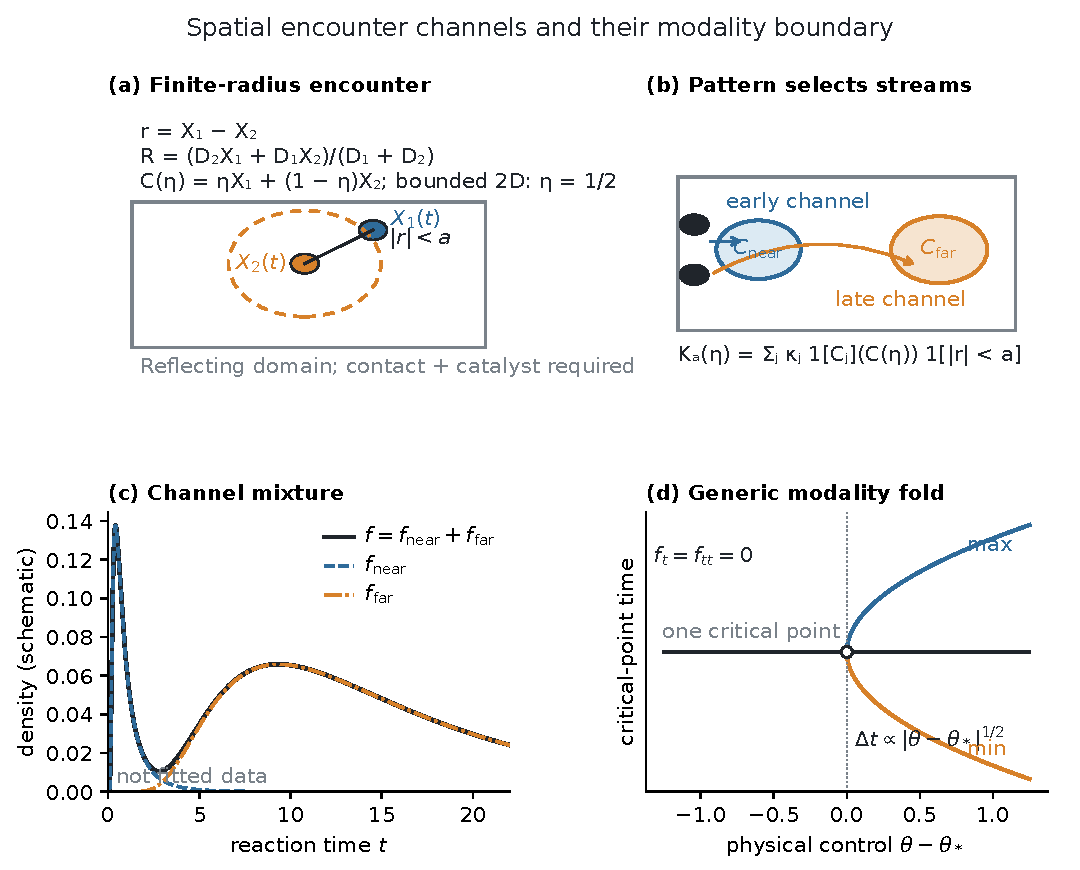
\includegraphics[width=6.65in]{encounter_model_and_fold}
\caption{\label{fig:model-fold}
Spatial encounter channels and their modality boundary. (a) Reaction requires
finite-radius contact and catalytic activation at a declared affine encounter
location. (b) Separated patches select early and late streams. (c) Their sum
can be bimodal; the curves are schematic and are not fitted data. (d) At a
generic fold, a maximum--minimum pair is created with square-root separation
under a physical control.}
\end{figure*}

\section{Finite encounter model and Green reduction}
\label{sec:green}

Let \(X_i(t)\in\Omega\subset\mathbb R^d\) be two independent particles before
reaction, with generator \(\Lfree\) and reflecting outer boundaries. A finite
contact radius \(a>0\) and an affine catalytic coordinate
\[
C_\eta(x_1,x_2)=\eta x_1+(1-\eta)x_2,\qquad 0\leq\eta\leq1,
\]
define channel killing fields
\begin{align}
K_{a,j}^{(\eta)}
&=\kappa_j(C_\eta)\mathbf 1_{C_j}(C_\eta)
\mathbf 1_{\{|x_1-x_2|<a\}},\notag\\
K_a^{(\eta)}&=\sum_jK_{a,j}^{(\eta)}.
\label{eq:doi-killing}
\end{align}
The unreacted joint density obeys
\begin{equation}
\partial_t p=\Lfree p-K_a^{(\eta)}p.
\label{eq:joint-fp}
\end{equation}
With \(S(t)=\int p\) and
\(f_j(t)=\int K_{a,j}^{(\eta)}p\), reflecting boundaries give the exact mass
balance
\begin{equation}
-S'(t)=f(t)=\sum_j f_j(t).
\label{eq:mass-balance}
\end{equation}
The catalyst coordinate is part of the physical model: the midpoint and the
diffusion-decoupling weighted centre are unequal when the particle
diffusivities differ. Coordinate algebra, the transformed domain, Doi--Robin
qualifications, and the finite-grid midpoint audit are given in the
Supplemental Material \cite{supplementalMaterial}.

Write the volume killing operator on
\(\mathsf H=L^2(\mathcal D)\) as
\begin{equation}
V=\Gamma^*\mathsf K\Gamma,\qquad
\Tgen=\Lfree-V,
\label{eq:killed-operator}
\end{equation}
where \(\Gamma\) restricts a function to the reaction support,
\(\Gamma^*\) extends it by zero, and \(\mathsf K\) is a bounded nonnegative
multiplication operator on that support. It may have a kernel. For
\({\rm Re}\,s\) above the spectral bound, define
\begin{equation}
\Rfree(s)=(s-\Lfree)^{-1},\qquad
\Gres(s)=\Gamma\Rfree(s)\Gamma^*.
\label{eq:restricted-green}
\end{equation}
Whenever the displayed inverse exists, the inverse-free resolvent identity is
\begin{equation}
(s-\Tgen)^{-1}
=\Rfree-\Rfree\Gamma^*\mathsf K
 (I+\Gres\mathsf K)^{-1}\Gamma\Rfree.
\label{eq:woodbury-operator}
\end{equation}
Thus, for \(u=\Gamma\Rfree q_0\), the restricted state and transformed
reaction density are
\begin{equation}
x=(I+\Gres\mathsf K)^{-1}u,\qquad
y=\mathsf K(I+\Gres\mathsf K)^{-1}u.
\label{eq:support-density}
\end{equation}
No inverse of \(\mathsf K\) is required. This separation exposes free
transport through \(\Gres\), geometry through \(\Gamma\), and intrinsic
chemistry through \(\mathsf K\).

For a finite continuous-time Markov chain (CTMC), adopt row vectors. Let
\(L_0=L_1\oplus L_2\), let columns of \(U\) select reactive states, and let
\(K\) be diagonal in channel rates. Then
\begin{equation}
T=L_0-UKU^\mathsf T,\qquad
f_j(t)=\alpha\e^{Tt}UKe_j.
\label{eq:finite-channel}
\end{equation}
The finite support matrix
\[
G(s)=U^\mathsf T(sI-L_0)^{-1}U
\]
gives
\[
\det(sI-T)=\det(sI-L_0)\det[I+G(s)K].
\]
The second determinant locates only candidate killed poles coupled to the
reaction support. Dark transport modes, numerator cancellation, and
observable residues must still be checked. Splitting probabilities are
computed from the stable killed solve
\begin{equation}
\bm\pi=\alpha(-T)^{-1}UK,
\label{eq:splitting-killed}
\end{equation}
when the reachable live chain is transient. Exact time derivatives are
\begin{equation}
\partial_t^n f(t)=\alpha\e^{Tt}T^nUK\bm1.
\label{eq:time-derivatives}
\end{equation}
The detailed two-site exclusion test model and zero-frequency diagnostics are
reported in the Supplemental Material \cite{supplementalMaterial}.

\section{Spectral gate and fixed-budget susceptibility}
\label{sec:modality-design}

\subsection{A necessary sign-variation condition}
\label{sec:spectral-bound}

Consider a finite killed model whose observable density has a real,
diagonalizable spectral expansion. After equal decay rates are grouped and
zero residues removed, write
\begin{equation}
f(t)=\sum_{j=1}^{n}a_j\e^{-\lambda_jt},
\qquad 0<\lambda_1<\cdots<\lambda_n.
\label{eq:spectral-density}
\end{equation}
Reversibility is a sufficient hypothesis because detailed balance makes the
killed generator similar to a real symmetric matrix. Applying the classical
generalized Descartes rule \cite{jameson2006descartes} to
\begin{equation}
f_t(t)=-\sum_{j=1}^{n}\lambda_ja_j\e^{-\lambda_jt}
\label{eq:spectral-derivative}
\end{equation}
after \(x=\e^{-t}\) gives the following corollary:
\[
\#\{\hbox{positive-time zeros of }f_t\}
\leq V(a_1,\ldots,a_n),
\]
where zeros are counted with multiplicity and \(V\) is the number of ordered
residue sign changes. Hence \(m\) nondegenerate interior maxima separated by
minima require
\begin{equation}
V(a_1,\ldots,a_n)\geq2m-1.
\label{eq:spectral-mode-bound}
\end{equation}
This is a necessary falsification gate, not a mode-count predictor. Three
sign changes can coexist with only one positive critical point, and a
rank-one killing support can already produce a bimodal phase-type density.
Reaction-support rank therefore cannot replace the observable residues.

Full symmetric eigendecompositions rebuild the two primary generators used in
the numerical audits. Reversibility, the gate's hypothesis, is verified
directly for both free generators: every live transition is two-way, a
spanning-tree reconstruction of the detailed-balance log-weights closes on
all off-tree edges with maximum cycle inconsistency \(2.4\times10^{-14}\)
(961 states) and \(9.1\times10^{-14}\) (2025 states), and the recovered
measure symmetrizes the killed generator. Equal decay rates are grouped at a
relative tolerance \(2\times10^{-10}\) before residues are summed; at that
tolerance no two eigenvalues of either generator merge. The 961-state finite
encounter generator is evaluated
at its three reported critical points; the separate 2025-state
three-channel generator is evaluated at five detected critical
points. Across the four relative residue cutoffs \(10^{-12}\), \(10^{-10}\),
\(10^{-8}\), and \(10^{-6}\) (relative to the summed absolute grouped
residues), the
minimum retained sign counts are 444 and 191, respectively, above the
necessary bounds three and five. Because these reconstructions reuse the
same generator constructors and critical-time artifacts, they test decomposition
and reconstruction rather than discover roots independently. Full cutoff,
counterexample, and reconstruction details are in the Supplemental Material
\cite{supplementalMaterial}.

\subsection{Budget-projected modality response}
\label{sec:budget-gradient}

For a finite live-state transport generator \(L\), let
\begin{equation}
T(k)=L-\operatorname{diag}k,\qquad
f(t;k)=\alpha\e^{T(k)t}k,
\label{eq:killing-design-model}
\end{equation}
where \(k>0\) on the allowed design support. For
\(k_\epsilon=k+\epsilon h\), put \(H=-\operatorname{diag}h\). The exact
Fr\'echet--Duhamel identity is
\begin{equation}
D\e^{Tt}[H]=\int_0^t\e^{T(t-s)}H\e^{Ts}\,\dd s
\label{eq:design-duhamel}
\end{equation}
\cite{alMohyHigham2009frechet}. Since
\(f_t=\alpha\e^{Tt}Tk\), its complete directional derivative is
\begin{equation}
D_kf_t(t;k)[h]
=\alpha D\e^{Tt}[H]Tk+\alpha\e^{Tt}(Hk+Th).
\label{eq:modality-susceptibility}
\end{equation}
The second term is essential because the killing field is also the measured
reaction observable. Writing this linear functional as \(g^\mathsf Th\),
\begin{equation}
g_i=(\alpha\e^{Tt}T)_i-k_i(\alpha\e^{Tt})_i
-\int_0^t(\alpha\e^{T(t-s)})_i(\e^{Ts}Tk)_i\,\dd s.
\label{eq:modality-gradient}
\end{equation}

Let \(c>0\) define the declared budget \(c^\mathsf Th=0\), and let
\(M\succ0\) define the local norm \(h^\mathsf TMh=1\). Put
\begin{equation}
\lambda_B=\frac{c^\mathsf TM^{-1}g}{c^\mathsf TM^{-1}c},
\qquad \widetilde g=g-\lambda_Bc.
\label{eq:budget-projection}
\end{equation}
Cauchy--Schwarz on the budget tangent space gives
\begin{equation}
h_*=\frac{M^{-1}\widetilde g}
{\sqrt{\widetilde g^\mathsf TM^{-1}\widetilde g}},
\qquad
\max D_kf_t[h]=\sqrt{\widetilde g^\mathsf TM^{-1}\widetilde g}.
\label{eq:optimal-redistribution}
\end{equation}
At a double stationary point, \(\widetilde g\ne0\) means that some
infinitesimal feasible redistribution is transverse to the fold. The
direction depends on the selected budget \(c\) and metric \(M\); it is not a
coordinate-free global optimum.

An eleven-state test model, with seeded random positive diagonal metric
\(M\) and budget vector \(c\) (uniform draws on \([0.65,1.85]\) and
\([0.55,1.65]\)), compares Eq.~\eqref{eq:modality-gradient} with a
basis Fr\'echet calculation, 256 independently generated budget-zero finite differences, a
state permutation, and 20,000 random feasible directions. The relative
Duhamel error is \(3.3\times10^{-15}\), the maximum independent finite-difference
error is \(2.4\times10^{-8}\), and the best random response is \(0.933\) of
Eq.~\eqref{eq:optimal-redistribution}. At the finite encounter fold below,
the chain-rule reconstruction of the computed log-rate transversality agrees
to \(6.8\times10^{-15}\) relative error. The orthogonal near-to-far
fixed-state-sum redistribution has nonzero transversality
\(-1.1621\times10^{-5}\).

\section{Physical folds in finite encounter generators}
\label{sec:fold-results}

At a fold of density critical points under a physical parameter \(\theta\),
\begin{equation}
f_t(t_*,\theta_*)=f_{tt}(t_*,\theta_*)=0.
\label{eq:physical-fold}
\end{equation}
The generic nondegeneracy conditions are
\begin{equation}
a_*=f_{t\theta}(t_*,\theta_*)\ne0,\qquad
b_*=f_{ttt}(t_*,\theta_*)\ne0.
\label{eq:fold-nondegenerate}
\end{equation}
Taylor expansion gives
\[
f_t=a_*\Delta\theta+\frac{b_*}{2}\Delta t^2+
o(|\Delta\theta|+|\Delta t|^2).
\]
On the side where \(-2a_*\Delta\theta/b_*>0\), the new maximum and minimum
separate as
\begin{equation}
\Delta t_\pm=
\pm\sqrt{-\frac{2a_*}{b_*}\Delta\theta}
+o(|\Delta\theta|^{1/2}),
\label{eq:fold-roots}
\end{equation}
and integrating the quadratic derivative gives prominence proportional to
\(|\Delta\theta|^{3/2}\). These equations concern a physical control that can
change both channel weights and shapes; a freely adjusted mixture weight is
not substituted for \(\theta\).

\subsection{Finite two-reactant CTMC certificate}
\label{sec:finite-ctmc}

The finite encounter chain has sites \(0,\ldots,30\). Its two independently
clocked walkers have interior total (attempt) jump rates \(0.7\) and \(0.2\),
respectively, and a common right bias \(0.3\). Their interior left/right rates
are therefore
\((0.245,0.455)\) and \((0.07,0.13)\). At a boundary an out-of-range jump is
omitted, giving the declared reflecting (holding) convention. If \(L_1\) and
\(L_2\) are the corresponding row generators, the free pair generator is the
Kronecker sum \(L_1\oplus L_2=L_1\otimes I+I\otimes L_2\), and the initial law
is concentrated at \((3,15)\). Killing acts only at the reactive co-locations
\((13,13)\) and \((30,30)\), with rates \(\kappa_{\rm near}\) and
\(\kappa_{\rm far}\), respectively. Transport and the initial law remain
fixed. We set \(\kappa_{\rm far}=-\log 0.4=0.9162907319\) and vary
\begin{equation}
\theta=\log(\kappa_{\rm near}/\kappa_{\rm far}),
\label{eq:ctmc-control}
\end{equation}
so that \(\kappa_{\rm near}=\kappa_{\rm far}e^\theta\). Parameter derivatives
are computed by propagating the column state and its sensitivity,
\begin{equation}
p'=T^\mathsf Tp,\qquad
s'=T^\mathsf Ts+T_\theta^\mathsf Tp,\qquad s(0)=0,
\label{eq:augmented-sensitivity}
\end{equation}
in one augmented matrix exponential; all semigroup actions are sparse
matrix-exponential actions in IEEE double precision. Time derivatives use
Eq.~\eqref{eq:time-derivatives}; no sampled-curve maximum is used to locate
the fold, which is obtained by a Powell hybrid root solve on the scaled
residual pair \((f_t,f_{tt})\) with parameter tolerance \(10^{-11}\) and
guarded acceptance thresholds.

The numerical root is
\begin{equation}
t_*=37.0749586402,\qquad
\theta_*=-9.6753635853,
\label{eq:ctmc-fold-point}
\end{equation}
corresponding to
\(\kappa_{\rm near}=5.755410148\times10^{-5}\). Residuals and margins are
made dimensionless with the fold time and density:
\(|f_t|t_*/f=7.1\times10^{-15}\),
\(|f_{tt}|t_*^2/f=6.8\times10^{-13}\), third derivative
\(f_{ttt}t_*^3/f=69.94\), and parameter transversality
\(f_{t\theta}t_*/f=-0.1962\). Independent continuation uses a symmetric
geometric ladder of fourteen control offsets
\(\Delta\theta=\pm0.001\)--\(0.064\) that play no role in locating the
fold; the log--log fits use the six two-peak-side offsets
\(\Delta\theta\le0.032\) and give slopes \(0.50095\) for separation and
\(1.50877\) for prominence, while the seven one-peak-side offsets confirm
the absence of any critical pair (Fig.~\ref{fig:gigfold}). The normal-form
amplitude is tested as well: the predicted separation
\(2\sqrt{-2a_*/b_*}\,\Delta\theta^{1/2}=5.554\,\Delta\theta^{1/2}\)
matches the measured separations to \(0.01\%\) at \(\Delta\theta=0.001\)
and \(0.7\%\) at \(\Delta\theta=0.064\). Mass closure is \(4.0\times10^{-15}\), and survival
at \(t=5000\) is \(1.3\times10^{-21}\).

\begin{figure*}[!t]
\centering
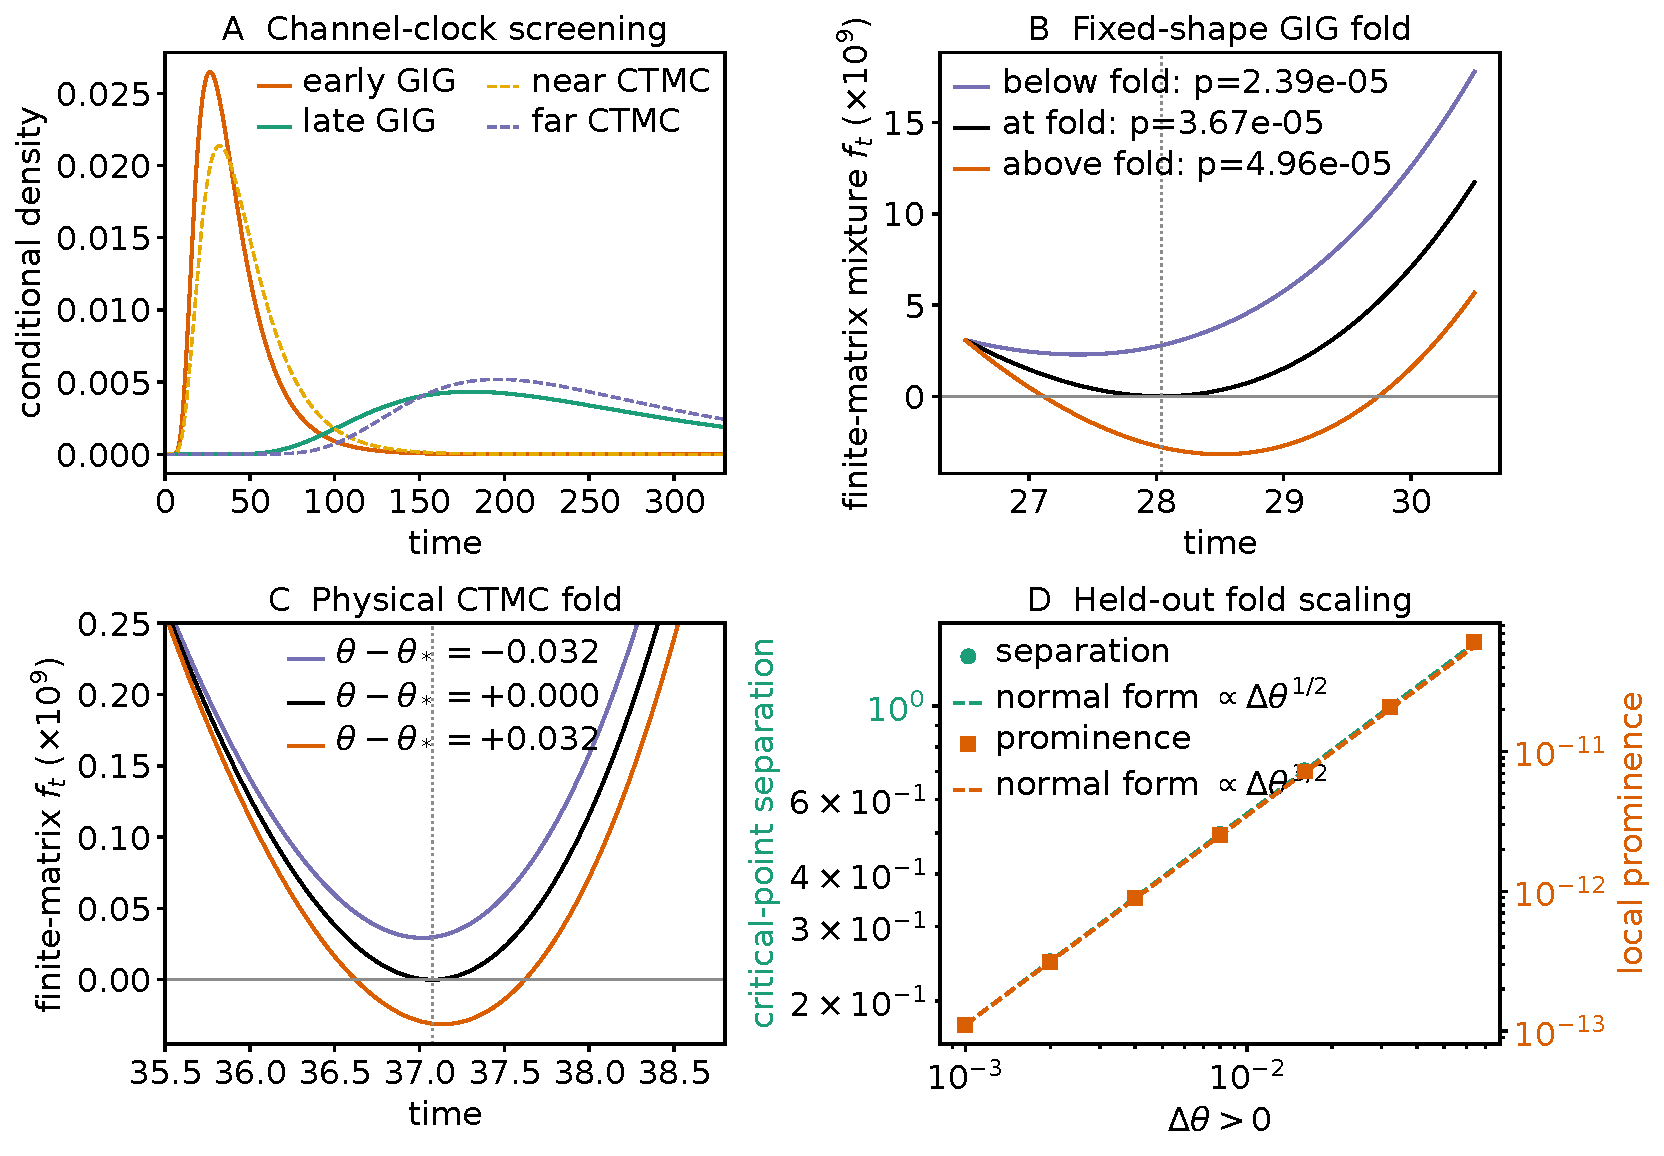
\includegraphics[width=6.65in]{gig_fold_validation}
\caption{\label{fig:gigfold}
Finite-CTMC fold certificate. The fold is located directly from
matrix-exponential derivatives of the killed generator. Independent continuation
recovers the \(1/2\) separation and \(3/2\) prominence exponents. The
free-space GIG channel clocks shown in the figure are screening estimates,
not replacements for the finite-matrix calculation; their derivation and
clock-control audits are in the Supplemental Material
\cite{supplementalMaterial}. The near-channel splitting probability at the
fold is \(8.95\times10^{-6}\), so the result establishes a mechanism rather
than two comparably observable streams.}
\end{figure*}

The very small near-channel probability is reported as a limitation. The
fold is derivative-certified even though the emerging feature is not a
practically balanced two-peak signal. The associated synchronous discovery,
Poissonized-clock comparison, and GIG approximation errors are secondary
mechanism checks and are kept in the Supplemental Material
\cite{supplementalMaterial}.

\subsection{Finite-radius two-dimensional matched-budget folds}
\label{sec:2d-fold-continuation}

The second family---labeled M2D-F, for matched-budget two-dimensional finite-radius---is a separate bounded realization. Two
particles evolve on the obstacle-free unit square with reflecting outer
boundaries. Each one-particle generator is a conservative boundary-node CTMC
with central nearest-neighbor diffusion, upwind longitudinal drift, and a
smooth transverse restoring drift: on the uniform grid with spacings
\(h_x,h_y\), a node jumps to its right or left neighbor at rate
\(D/h_x^2+\max(\pm v_x,0)/h_x\) and to its upper or lower neighbor at rate
\(D/h_y^2+\max(\pm v_y,0)/h_y\), with drift field
\((v_x,v_y)=(v,\,-\gamma_\perp(y-\tfrac12))\), and out-of-range jumps are
omitted (reflection by omission). Reaction occurs when the particle
separation is at most \(a=0.17\) and the midpoint
\(C_{1/2}=(X_1+X_2)/2\) lies in one of two circular catalytic patches.
The parameters are
\[
(D_1,v_1)=(0.0025,0.115),\qquad
(D_2,v_2)=(0.0008,0.02),
\]
with transverse confinement \(1.5\), starts \((0,0.5)\) and
\((0.28,0.5)\), and near/far patch specifications
\begin{align*}
(x,r,\kappa)_{\rm near}&=(0.25,0.18,0.5),\\
(x,r,\kappa)_{\rm far}&=(0.72,0.20,15),
\end{align*}
where both patch centers have \(y=0.5\). The full closed-mask convention,
contact-safe initial-law construction, and dimensional scaling are specified
in the Supplemental Material \cite{supplementalMaterial}. Because the tested
grids have large local P\'eclet numbers and binary supports, they are treated
as finite generators rather than a controlled SDE refinement.

On each grid, a homogeneous rate \(\bar\kappa_h\) is recomputed so that the
unweighted statewise killing sum equals that of the patterned endpoint. The
reactive-tube state counts and matched rates are
\((N_T,N_{\rm near},N_{\rm far},\bar\kappa_h)=(125,7,9,1.108)\),
\((349,34,40,1.768)\), and \((1123,109,137,1.878)\) on the
\(9\times5\), \(11\times7\), and \(13\times9\) grids, and the build
aborts unless the killing sum at both path endpoints matches the budget to
\(2\times10^{-12}\). The
physical path is
\begin{equation}
\kappa_\theta(C_{1/2})=(1-\theta)\bar\kappa_h
+\theta\kappa_{\rm pat}(C_{1/2}),
\qquad 0\leq\theta\leq1.
\label{eq:2d-budget-path}
\end{equation}
Thus the discrete state-sum killing budget is fixed to roundoff while both
splitting weights and conditional channel shapes may vary. M2D-F is not a
continuation of the endpoint family M2D-E in the Supplemental Material:
transport parameters, reaction radius, starts, and per-grid budget paths
differ.

Sparse generator actions give \(f_t,f_{tt},f_{ttt}\), and an augmented
exponential gives the parameter derivatives; the fold system is solved with
its analytic \(2\times2\) Jacobian at parameter tolerance \(10^{-11}\),
under the same normalized acceptance guards as the encounter chain. The three physical-interval
folds are
\begin{align}
(t_c,\theta_c)_{9\times5}&=(16.8093321,0.27537300),\notag\\
(t_c,\theta_c)_{11\times7}&=(18.0995323,0.01381035),\notag\\
(t_c,\theta_c)_{13\times9}&=(16.5807587,0.25589201).
\label{eq:2d-folds}
\end{align}
The \(9\times5\) residuals are below \(3.5\times10^{-17}\), with
\(f_{ttt}=-1.34\times10^{-5}\) and
\(f_{t\theta}=1.67\times10^{-4}\). The \(11\times7\) residual pair is
\((8.7\times10^{-19},3.5\times10^{-18})\), with
\(f_{ttt}=-7.81\times10^{-6}\) and
\(f_{t\theta}=2.83\times10^{-4}\). The \(13\times9\) residuals are below
\(2.8\times10^{-17}\), with \(f_{ttt}=-5.96\times10^{-6}\) and
\(f_{t\theta}=7.46\times10^{-5}\).

Independent continuation from eight control offsets
\(\mu=\theta-\theta_c\in[2\times10^{-4},0.05]\), fitted on the six
offsets \(\mu\le0.01\), gives separation/prominence exponents
\((0.4989,1.5001)\), \((0.4933,1.4843)\), and
\((0.4993,1.5039)\). All three generators therefore satisfy the local
nondegenerate normal form. They do not form a convergent critical-control
sequence: the state-count-matched \(\theta_c\) values are nonmonotone and span
\(0.262\). Replacing equal node weights in the budget by tensor-product
boundary trapezoidal weights (per-axis weight \(\tfrac12\) on the two
boundary nodes and \(1\) in the interior, tensorized over both particles),
without changing the CTMC generators or masks,
moves the folds to \(0.6244,0.2408,0.4593\), again nonmonotonically, with span
\(0.384\). This one-factor audit shows that the finite-model fold is also
sensitive to the budget measure.

\begin{figure*}[!t]
\centering
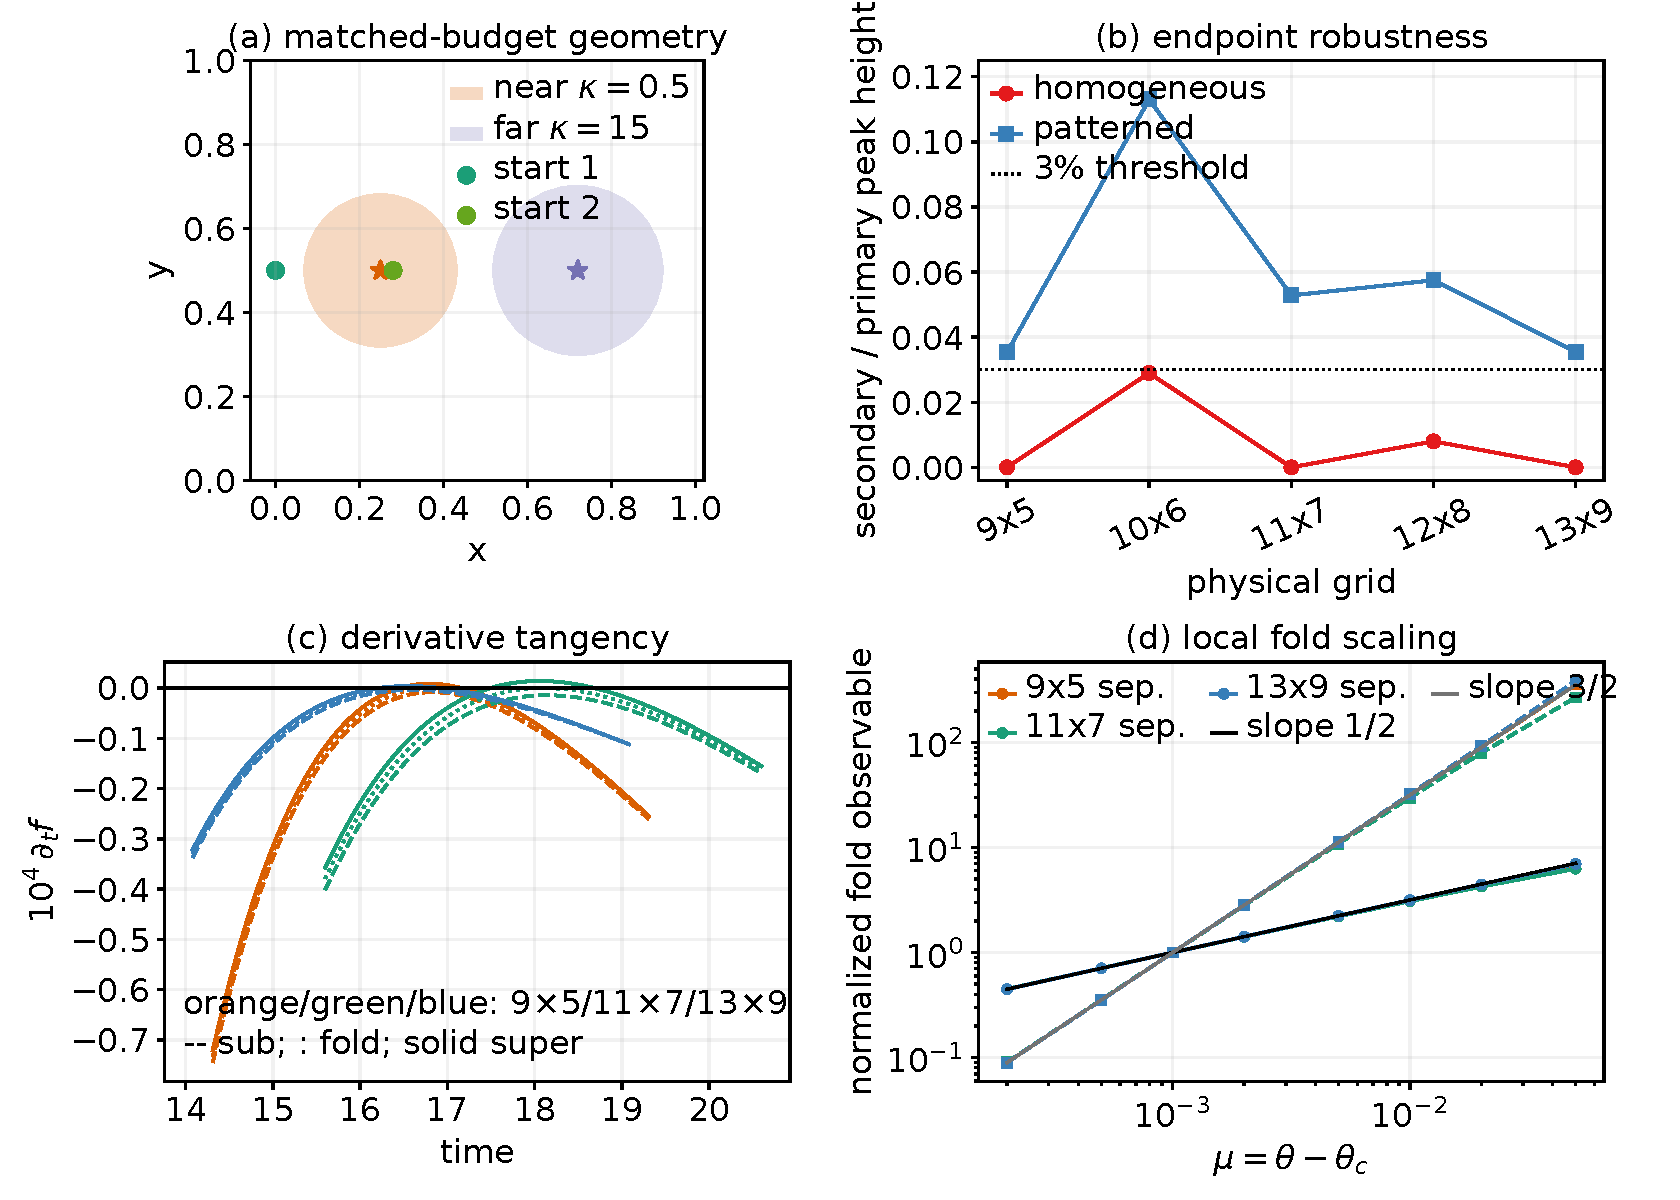
\includegraphics[width=6.65in]{finite_radius_2d_fold_validation}
\caption{\label{fig:2d-fold}
Finite-radius two-dimensional matched-budget (M2D-F) fold certificate. (a) Spatial
redistribution keeps the statewise killing sum fixed on each grid. (b) The
endpoint audit distinguishes resolved secondary peaks from reported
subthreshold ripples. (c) Analytic derivatives locate a tangency and its
two-sided continuations on three finite grids. (d) Each grid recovers square-root
separation and \(3/2\) prominence. The critical controls
\(0.275,0.014,0.256\) are explicitly nonmonotone and move under a second
budget measure; they are not estimates of a continuum fold.}
\end{figure*}

Figure~\ref{fig:2d-fold} collects the fixed-budget construction, the
endpoint morphology audit, the derivative-located folds, and their independent
normal-form scaling.

The two intervening grids are consistent with that caution. On
\(12\times8\), a nondegenerate continuation root lies at
\((t_c,\theta_c)=(18.26877,-0.06158)\), outside the physical path. On
\(10\times6\), a curvature scan over \(\theta\in[-0.2,0.1]\),
\(t\in[0.01,40]\) and four bounded least-squares starts (bounds
\(t\in[8,25]\), \(\theta\in[-0.2,0]\))
find no fold, with all starts reaching the same positive near miss
\(f_t=3.8721\times10^{-6}\). This bounded search does not cover the
interval \(\theta\approx0.25\)--\(0.28\) in which two of the three located
folds sit; it is a bounded diagnostic, not evidence of absence. Detailed endpoint roots, budget
quadrature, even-grid scans, and morphology settings are provided in the
Supplemental Material \cite{supplementalMaterial}.

\section{Discussion and scope}
\label{sec:discussion}

The finite-model calculation separates three questions. Transport determines
which temporal scales are available. The initial and reaction observables
determine the signs and amplitudes of their spectral residues. Finally, a
declared feasible reaction-field perturbation determines whether the
critical-point equation can be crossed. Patch count alone addresses none of
these questions: a support-rank-one counterexample can already be bimodal,
whereas a residue sequence with three sign changes need not have three
positive derivative roots.

The Green reduction and sensitivity calculus play complementary roles.
\(\Gres(s)\) reduces transport to the reaction support, while
Eqs.~\eqref{eq:modality-susceptibility}--\eqref{eq:optimal-redistribution}
operate directly on the time-domain fold equation. A killed pole can be dark
or cancel from a selected observable, and a density fold is not a spectral
exceptional point. The spectral sign count is therefore used only to
falsify an impossible finite reversible mode count, never to replace direct
time-derivative root calculations.

The finite encounter CTMC confirms the derivative chain but has a very small
minority channel. The M2D-F result more directly tests spatial redistribution
at a fixed per-grid budget, yet its grid and budget-measure sensitivity
prevents a continuum interpretation. The supporting Supplemental Material
shows additionally that spatial patterning can promote an existing
subthreshold maximum across an operational resolution threshold in a separate
endpoint family, but is not necessary for bimodality; a uniformly reactive
finite model provides a counterexample \cite{supplementalMaterial}. It also
records catalytic-coordinate sensitivity and underresolved three-patch
finite-grid examples. Those controls restrict causal language rather than
broaden the principal claim.

The main unresolved step is a continuum bridge. Preservation of already
simple modes needs derivative margins, whereas transfer of a nondegenerate
fold needs convergence of
\[
H_h=(\partial_t f_h,\partial_{tt}f_h)
\]
and its time/control Jacobian near the critical point. Joint local \(C^3\)
convergence in time and control is sufficient. Mere \(C^2\) convergence of
the densities is not sufficient because third time derivatives can lose
nondegeneracy. A cell-averaged, successively refined continuation with stable
support quadrature, extrapolated critical control, and convergent
parameter-Duhamel derivatives is therefore required before a continuum fold
can be claimed.

Other limits remain explicit. The projected optimum is local and ignores
finite-amplitude nonnegativity, box constraints, binary supports, and
nonsmooth patch motion. The Green identity is a right-half-plane
volume-reaction statement under its operator hypotheses; an unqualified
Robin trace analogue and continuum meromorphic continuation are not supplied.
The 2D grids use upwind transport and binary masks, and no independent Robin
or Brownian solver validates the fold. The chosen discrete state-sum budget
does not equalize pathwise hazards, splitting probabilities, or mean
lifetimes. Capacity and GIG calculations in the Supplemental Material are
calibration and screening layers, not centre-patterned modality theorems.

\section{Conclusions}
\label{sec:conclusions}

For a declared finite encounter generator, the observable spectral residues
give a necessary sign-variation gate, and the Fr\'echet--Duhamel derivative
gives the exact local response of the critical-point equation to the killing
field. Projection onto a budget tangent space then identifies the steepest
unit feasible redistribution in a chosen metric. These statements link
transport, reaction observability, and admissible control without equating
the number of catalytic patches with the number of modes.

Two numerical certificates exercise the calculus. A finite two-reactant CTMC
has a nondegenerate density fold with direct residual and transversality
checks and the expected continuation exponents. A separate finite-radius M2D-F
path has analogous folds on three finite grids under an exactly fixed
per-grid killing sum. Their critical controls are nonmonotone and
budget-measure sensitive, so the result stops at a finite-generator mechanism
certificate. Establishing a continuum fold requires a new convergence
calculation; it is not inferred from the present grids.

\section*{Data Availability}

The source code, numerical tables, vector figures, and machine-readable
provenance manifests that reproduce every reported number are available from
the author upon reasonable request, and will accompany the published article
as a public, versioned archive.

\bibliography{references}

\end{document}
